\documentclass{article}
\usepackage{float}
\usepackage{hyperref}
\usepackage{graphicx} % Required for inserting images
\usepackage[english]{babel}
\usepackage[T1]{fontenc}
\usepackage{textcomp}
%\usepackage{titlesec}
\usepackage{parskip}
\usepackage[margin=1in]{geometry}
\usepackage{color}

\graphicspath{{../figures/figures_report_2/}}

\title{ANALYSIS OF COVID-19 CHEST X-RAYS: Report 2: Modeling Report}
\author{Saniya Arfin, Yvonne Breitenbach, Alexandru Buzgan}
\date{May 2025}

\begin{document}

\maketitle

\tableofcontents

\newpage 

\section{Introduction}

\begin{itemize}
    \item \colorbox{yellow}{What kind of machine learning problem is your project like? (classification of images with 4 classes}
    \item \colorbox{yellow}{We first tried to solve the problem by using several machine learning methods}
    \item \colorbox{yellow}{Then tried Deep learning, DNNs, transfer laerning, ...}
    \item \colorbox{yellow}{What task does your project relate to? (fraud detection, facial recognition, sentiment analysis, etc)?}
    \item ...
\end{itemize}

\section{Machine Learning}

\subsection{Preprocessing Pipeline for Machine Learning}
The following subsections describe the different stages of preprocessing the data has run through before it was used for modelling.
\subsubsection{Input}
Input: Raw Images (299x299 RGB)
A set of raw images, each with dimensions 299x299 pixels, with 3 color channels (RGB) and some L.

\subsubsection{Convert to Grayscale}
Input: Raw images of size 299x299 RGB (colored images).\\
Operation: Convert the images from RGB (3 channels) to grayscale (single channel). This reduces the complexity and focus on intensity patterns.\\
Output: Images of size 299x299, but now with only 1 channel (grayscale). These images are binary-like in the sense that they only have intensity values rather than color.

\subsubsection{Apply Gaussian Blur to images}
Input: Grayscale images of size 299x299.\\
Operation: A Gaussian blur is applied to smooth the images and reduce noise. This blurring operation makes the image less sharp but removes high-frequency noise.\\
Output: Grayscale images of size 299x299, but with smoothed details and reduced noise.\\

\subsubsection{Contrast Enhancement with CLAHE}
Input: Grayscale images of size 299x299 to which Gaussian Blur filter has been applied.\\
Operation: CLAHE (Contrast Limited Adaptive Histogram Equalization) enhances the contrast of the images by redistributing the intensity values, making small details more prominent.\\
Output: Grayscale images of size 299x299, but with improved contrast.\\

\subsubsection{Normalization}
Input: Grayscale images of size 299x299, to which Gaussian Blur and CLAHE filter have been applied, with pixel values ranging from 0 to 255.\\
Operation: Normalize the pixel values to the range [0, 1] by dividing each pixel value by 255.\\
Output: Grayscale images of size 299x299, but with pixel values now in the range [0, 1]. The values are floating-point numbers.\\

\subsubsection{Resize the masks}
The masks have a size of 256x256 pixels and therefore cannot be combined with the X-ray images which have a size of 299x299 pixels. 
That is why the masks have been resized to 299x299 pixels.

\subsubsection{Convert masks to binary images}
The masks have been converted into binary images. 

\subsubsection{Combine masks with images:}
Each of the so far processed images havs been combined with its corresponding mask. This has been done by using the function "bitwise\_and" of the cv2-library.\\

\subsubsection{Pixel Value Normalization}
    \colorbox{yellow}{ToDo: write text}
    
\subsubsection{Label encoding}
Input: Class labels like "COVID", "Normal", "Lung Opacity", "Viral Pneumonia".\\
Operation: Convert categorical class labels into numeric labels using LabelEncoder (e.g., "COVID" = 0,"Lung Opactiy" = 1, "Normal" = 2, "Viral Pneumonia" = 3 ).\\
Output: Encoded labels as numeric values, stored in an array (e.g., [0, 1, 0, 2 ,...] for the respective classes).\\

\subsubsection{Split data into training and testing}
Input: Normalized images (of size 299x299) and encoded labels.\\
Operation: Split the data into training and testing sets, 80\% for training and 20\% for testing. We used the paramter "random\_state" of the function 
"sklearn.model\_selection.train\_test\_split" to make sure that the split is reproducable and we use the same train and test sets for working with the differend models.\\
As we have an imbalanced number of images in the different classes, we used the parameter "stratify" of the function "sklearn.model\_selection.train\_test\_split". This
ensures that the train and test datasets have the same proportion of classes as the original dataset. The class imbalance will be fixed in the train dataset later.\\
Output: Two datasets:
\begin{itemize}
    \item Training set: Images (normalized) and labels (encoded).
    \item Testing set: Images (normalized) and labels (encoded)
\end{itemize}

\subsubsection{Address Class Imbalance by Data Augmentation}
Since the distribution between the classes is not balanced (for example Viral Pneumonia images are far less numerous than the Normal images) we have to address this problem 
before the training stage. Appropriate strategies can be applied, such as:
\begin{itemize}
    \item Class weighting during model training
    \item Oversampling/undersampling
    \item Data augmentation for minority classes
\end{itemize}
This ensures the model does not become biased toward the majority classes and maintains fair performance across all categories. For our dataset (which consist of images) data augmentation is the most suited.

Input: Training dataset \\%with normalized images (of size 299x299).\\
Operation: Apply augmentation techniques like rotation and shifting to artificially increase number of images in the minority classes "COVID", "Lung Opacity" and "Viral Pneumonia".\\
Output: Augmented images, which are variations of the original images, still of size 299x299. These augmented images are then used to train the model more robustly.\\
\colorbox{yellow}{ToDo: Yvonne insert a graph with examples of augmented images.}\\
\colorbox{yellow}{ToDo: Yvonne insert table to show how many images we have per class before and after.}

\subsubsection{Feature Extraction}
Since we have a large dataset consisting of a total of 35059 images just in the train set it is a good idea to identify important features to reduce the computing time.
Extracting features reduces the image's size dramatically and converts it into a compact representation that's suitable for machine learning models. 

Chest X-ray images reveal structural differences in the lungs based on the condition. For example:
\begin{itemize}
    \item COVID-19 often shows bilateral ground-glass opacities.
    \item Viral / Bacterial Pneumonia can show localized consolidation or patchy opacities.
    \item Lung Opacity is a broader label that includes a range of conditions affecting lung transparency.
    \item Normal lungs have well-defined, clear lung fields.
\end{itemize}

\vspace{0.5cm}

To classify these visually distinct conditions, we need a way to extract structural patterns from grayscale X-ray images.\\

\noindent \underline{HOG:}
\vspace{0.5cm}\\
HOG, or Histogram of Oriented Gradients, is a feature descriptor used in computer vision and image processing.  
HOG captures the structure and edge directions in an image, which are crucial for identifying shapes and patterns.
\\

HOG Captures from X-rays

\begin{itemize}
     \item Edges of lung boundaries, rib cage, and lesions.
     \item Orientation and distribution of densities — darker/lighter areas correspond to tissue and opacity differences.
     \item Shape and spread of abnormalities, like how diffuse or sharp an opacity is.
\end{itemize}
Although HOG is handcrafted, not learned  and  so it may miss subtle texture or high-level patterns, it is a fast, interpretable, and memory-efficient way to 
extract features from chest X-rays. \\
We have a HOG (Histogram of Oriented Gradients) feature dataset with a shape of (35059, 8100), which means:
\begin{itemize}
    \item 35059 represents the number of images in your dataset.
    \item 8100 represents the number of features extracted from each image using the HOG method.
\end{itemize}
	
These 8100 features are typically a flattened representation of the gradients and orientations from the original image. Our image was originally a 299x299 
pixel image, the HOG algorithm works by breaking the image into smaller cells (e.g., 8x8 pixels per cell), compute the gradient orientations, 
and then describe the image based on these features. The 8100 features might correspond to a smaller, downscaled version of the original image, where each image
is transformed into a set of descriptive gradient-based features, rather than keeping the full raw pixel values.
In simpler terms, we are working with feature vectors derived from each image, not the full size of the image. Each of the 8100 features corresponds to a 
particular characteristic (such as the gradient of pixel intensity) of the image after applying the HOG technique.
So, (35059, 8100) indicates that we have 35059 images, and each image has been transformed into a feature vector of length 8100 after HOG processing.

\begin{figure}[h!] % the [h!] helps force it "here"
    \centering
    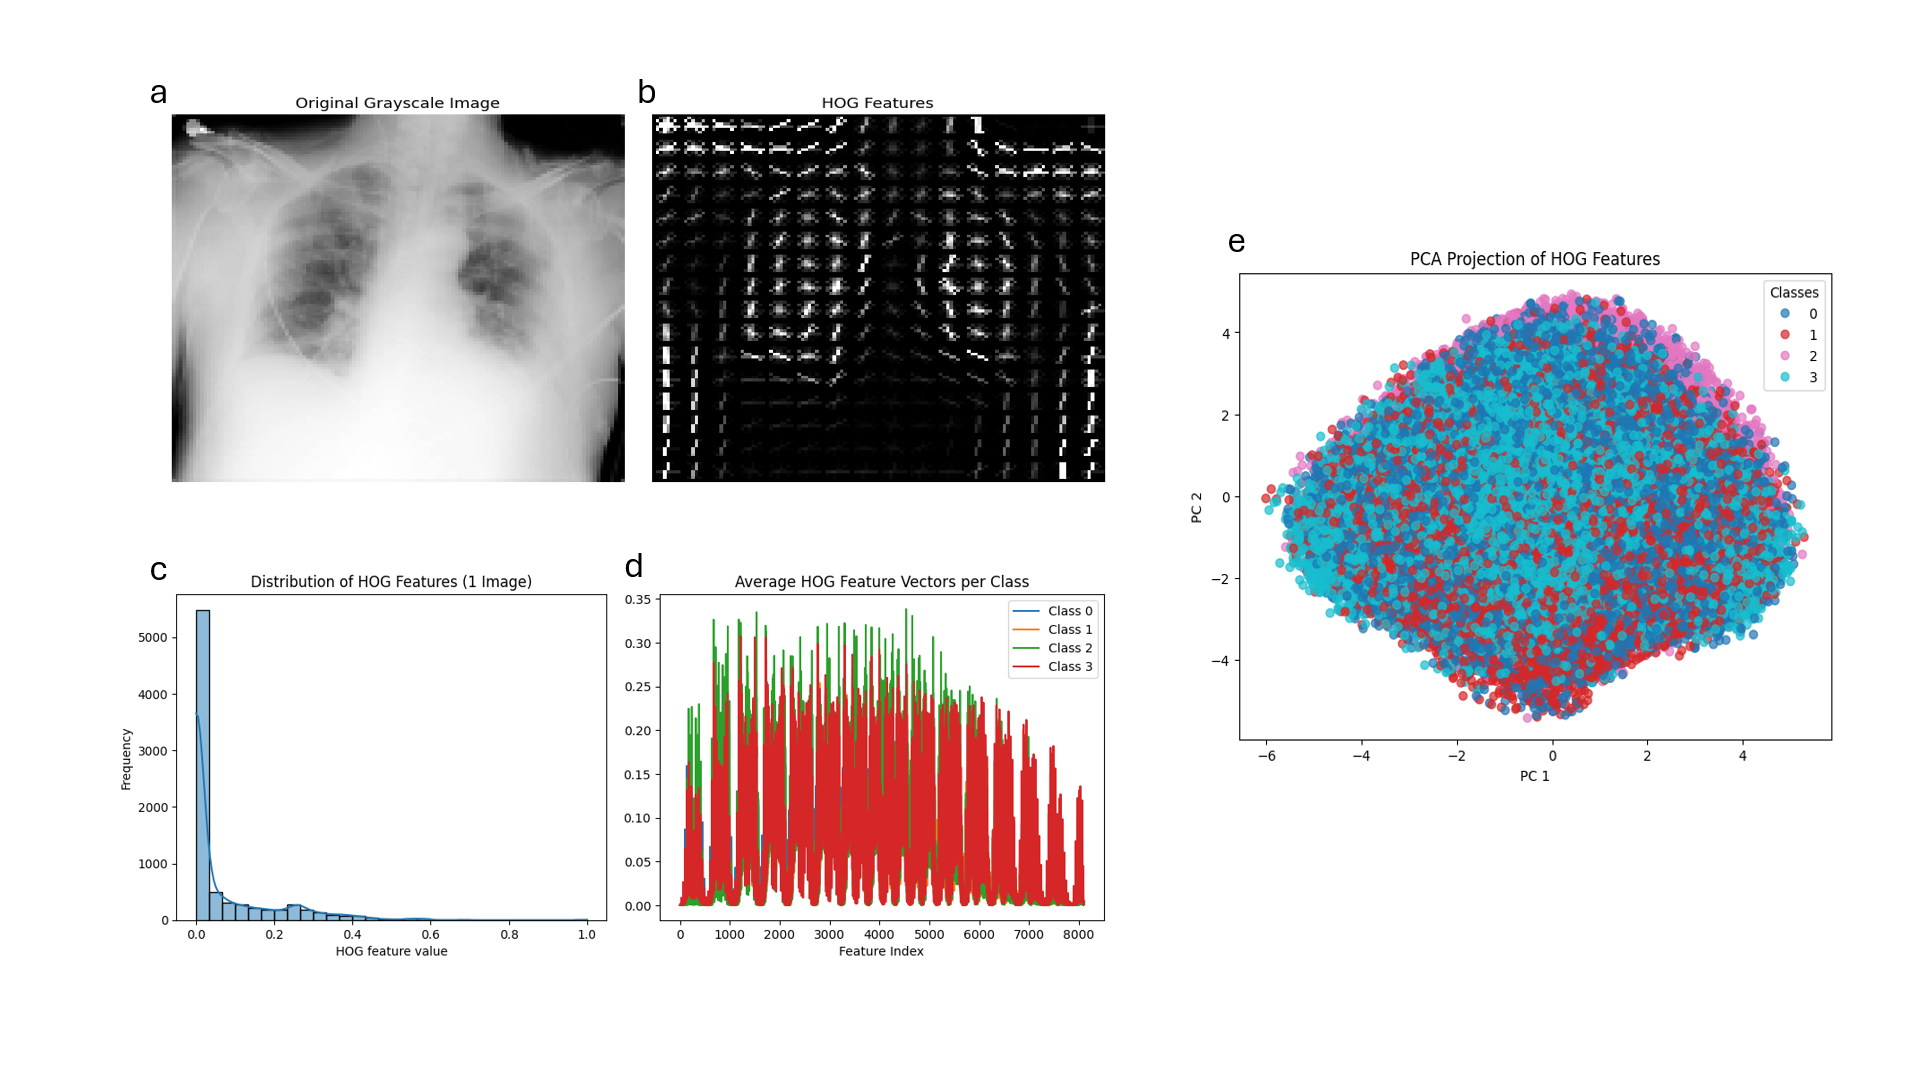
\includegraphics[width=1.0\linewidth]{hogfeatures_all.png}
    \caption{Visualisation of hog features}
    \label{fig:Visualisation of hog features}
\end{figure}
Figure \ref{fig:Visualisation of hog features}a shows the original grayscale image. We can clearly see the chest X-ray with anatomical structures 
like ribs and lungs.\\
Figure \ref{fig:Visualisation of hog features}b effectively displays edges and gradients, especially around the rib cage, clavicle, and lung boundaries. 
The blocky structure is normal due to the cell/block division of the HOG algorithm (e.g., 8x8 pixels per cell). The highlighted edges capture shape and 
orientation information, which HOG is designed to emphasize. The features look rich and well-distributed and are therefore useful for capturing structural patterns:\\
Figure \ref{fig:Visualisation of hog features}c displays the distribution of HOG Features per image. Most feature values are near zero (common in HOG due 
to sparse gradients) in the histogram and a long tail which represents stronger edges or corners.\\
The line plot shows the average HOG values across feature indices for each class used for class separability analysis 
(Figure \ref{fig:Visualisation of hog features}d). It helps identify which feature indices (spatial areas or orientations) contribute more for specific classes. 
Overlapping curves indicate similar structures between some classes (e.g., viral vs lung opacity).\\
We also plot a PCA projection of HOG characteristics (figure \ref{fig:Visualisation of hog features}e). The 2D scatter plot of HOG characteristics 
after reduction of dimensionality using PCA (Principal Component Analysis) showed significant overlap suggesting that HOG alone may not strongly separate 
some classes (hence the need for a classifier).
In summary, HOG works well visually, but it’s not sufficient alone for strong class separation in our dataset. Therefore for most our ML models, 
we use HOG features but we also extracted deeper features using other methods like ResNet, VGG16 and GLCM.
\\

\vspace{0.5cm}
    

\underline{VGG:}\\
\colorbox{yellow}{infos and results for VGG-method}
\\

\underline{other:}\\
\colorbox{yellow}{infos and results for another method we tried}
\\

\underline{combined methods:}
infos and results for a combination of methods

\colorbox{yellow}{I don't understand if the following itemize another subsebsection or does it belong to the subsubsection "feature extraction"?}
\begin{itemize}
    \item Flatten Features for ML Models\\
    Input: Extracted HOG features (1D numpy array) for each image.\\
    Operation: Flatten the 2D image representation into a single 1D array of features.\\
    Output: A 1D numpy array for each image that can be used as input to machine learning models. This would typically be an array of shape (n\_samples, n\_features).\\
    \item Training Machine Learning Models:\\
    Input: Feature arrays (flattened HOG features) and encoded labels.
    Operation: Use machine learning models (e.g.Random Forest, Logistic Regression, XGBoost) to train on the feature vectors.
    Output: A trained model that can predict the class (label) of new, unseen images based on their feature vectors.
\end{itemize}


\subsection{Metrics to Evaluate the Model Results}
Input: Trained machine learning model and the test set (augmented images, labels).\\
Operation: Evaluate the model's performance using metrics like accuracy, F1 score, and confusion matrix to understand how well it classifies the different 
image classes.\\
Output: Evaluation metrics to show true vs predicted labels.

There are also a number of hyperpramater tuning strategies, which are summarized below:
\begin{table}[ht]
    \centering
    \renewcommand{\arraystretch}{1.3}
    \begin{tabular}{|c|c|p{8cm}|}
        \hline
        \textbf{Method} & \textbf{Recommended For Us?} & \textbf{Why} \\ \hline
        GridSearchCV & No & Too slow for SVMs (due to image data + multiple classes) \\ \hline
        RandomizedSearchCV & Yes & A great starting point. Fast, simple, and well-suited for ML models like SVM, k-NN, RF \\ \hline
        BayesSearchCV & Yes & \textbf{(Advanced)} Ideal for tuning deep models (CNNs) or complex ML pipelines with many parameters — faster than Grid, smarter than Random \\ \hline
    \end{tabular}
    \caption{Comparison of hyperparameter tuning strategies}
    \label{tab:tuning_methods}
\end{table}

Table \ref{tab:tuning_methods} shows \dots
We used the following hyperparameter optimization strategies: \\
\colorbox{yellow}{We have to work on this! Write down what we really used @Alex @Saniya @Yvonne}
\begin{itemize}
    \item RandomizedSearchCV for machine learning models (SVM, RandomForest)as it balances speed and accuracy well.
    \item BayesSearchCV: tried it for SVM. For deep learning models, especially CNNs, we can be efficient with GPU/CPU time, and so we will use it.
    \item We tired to work with GridSearchCV but its too slow on our large dataset and so not.
\end{itemize}


\subsection{Modelling and Results}
\begin{figure}%[ht] % the [h!] helps force it "here"
    \centering
    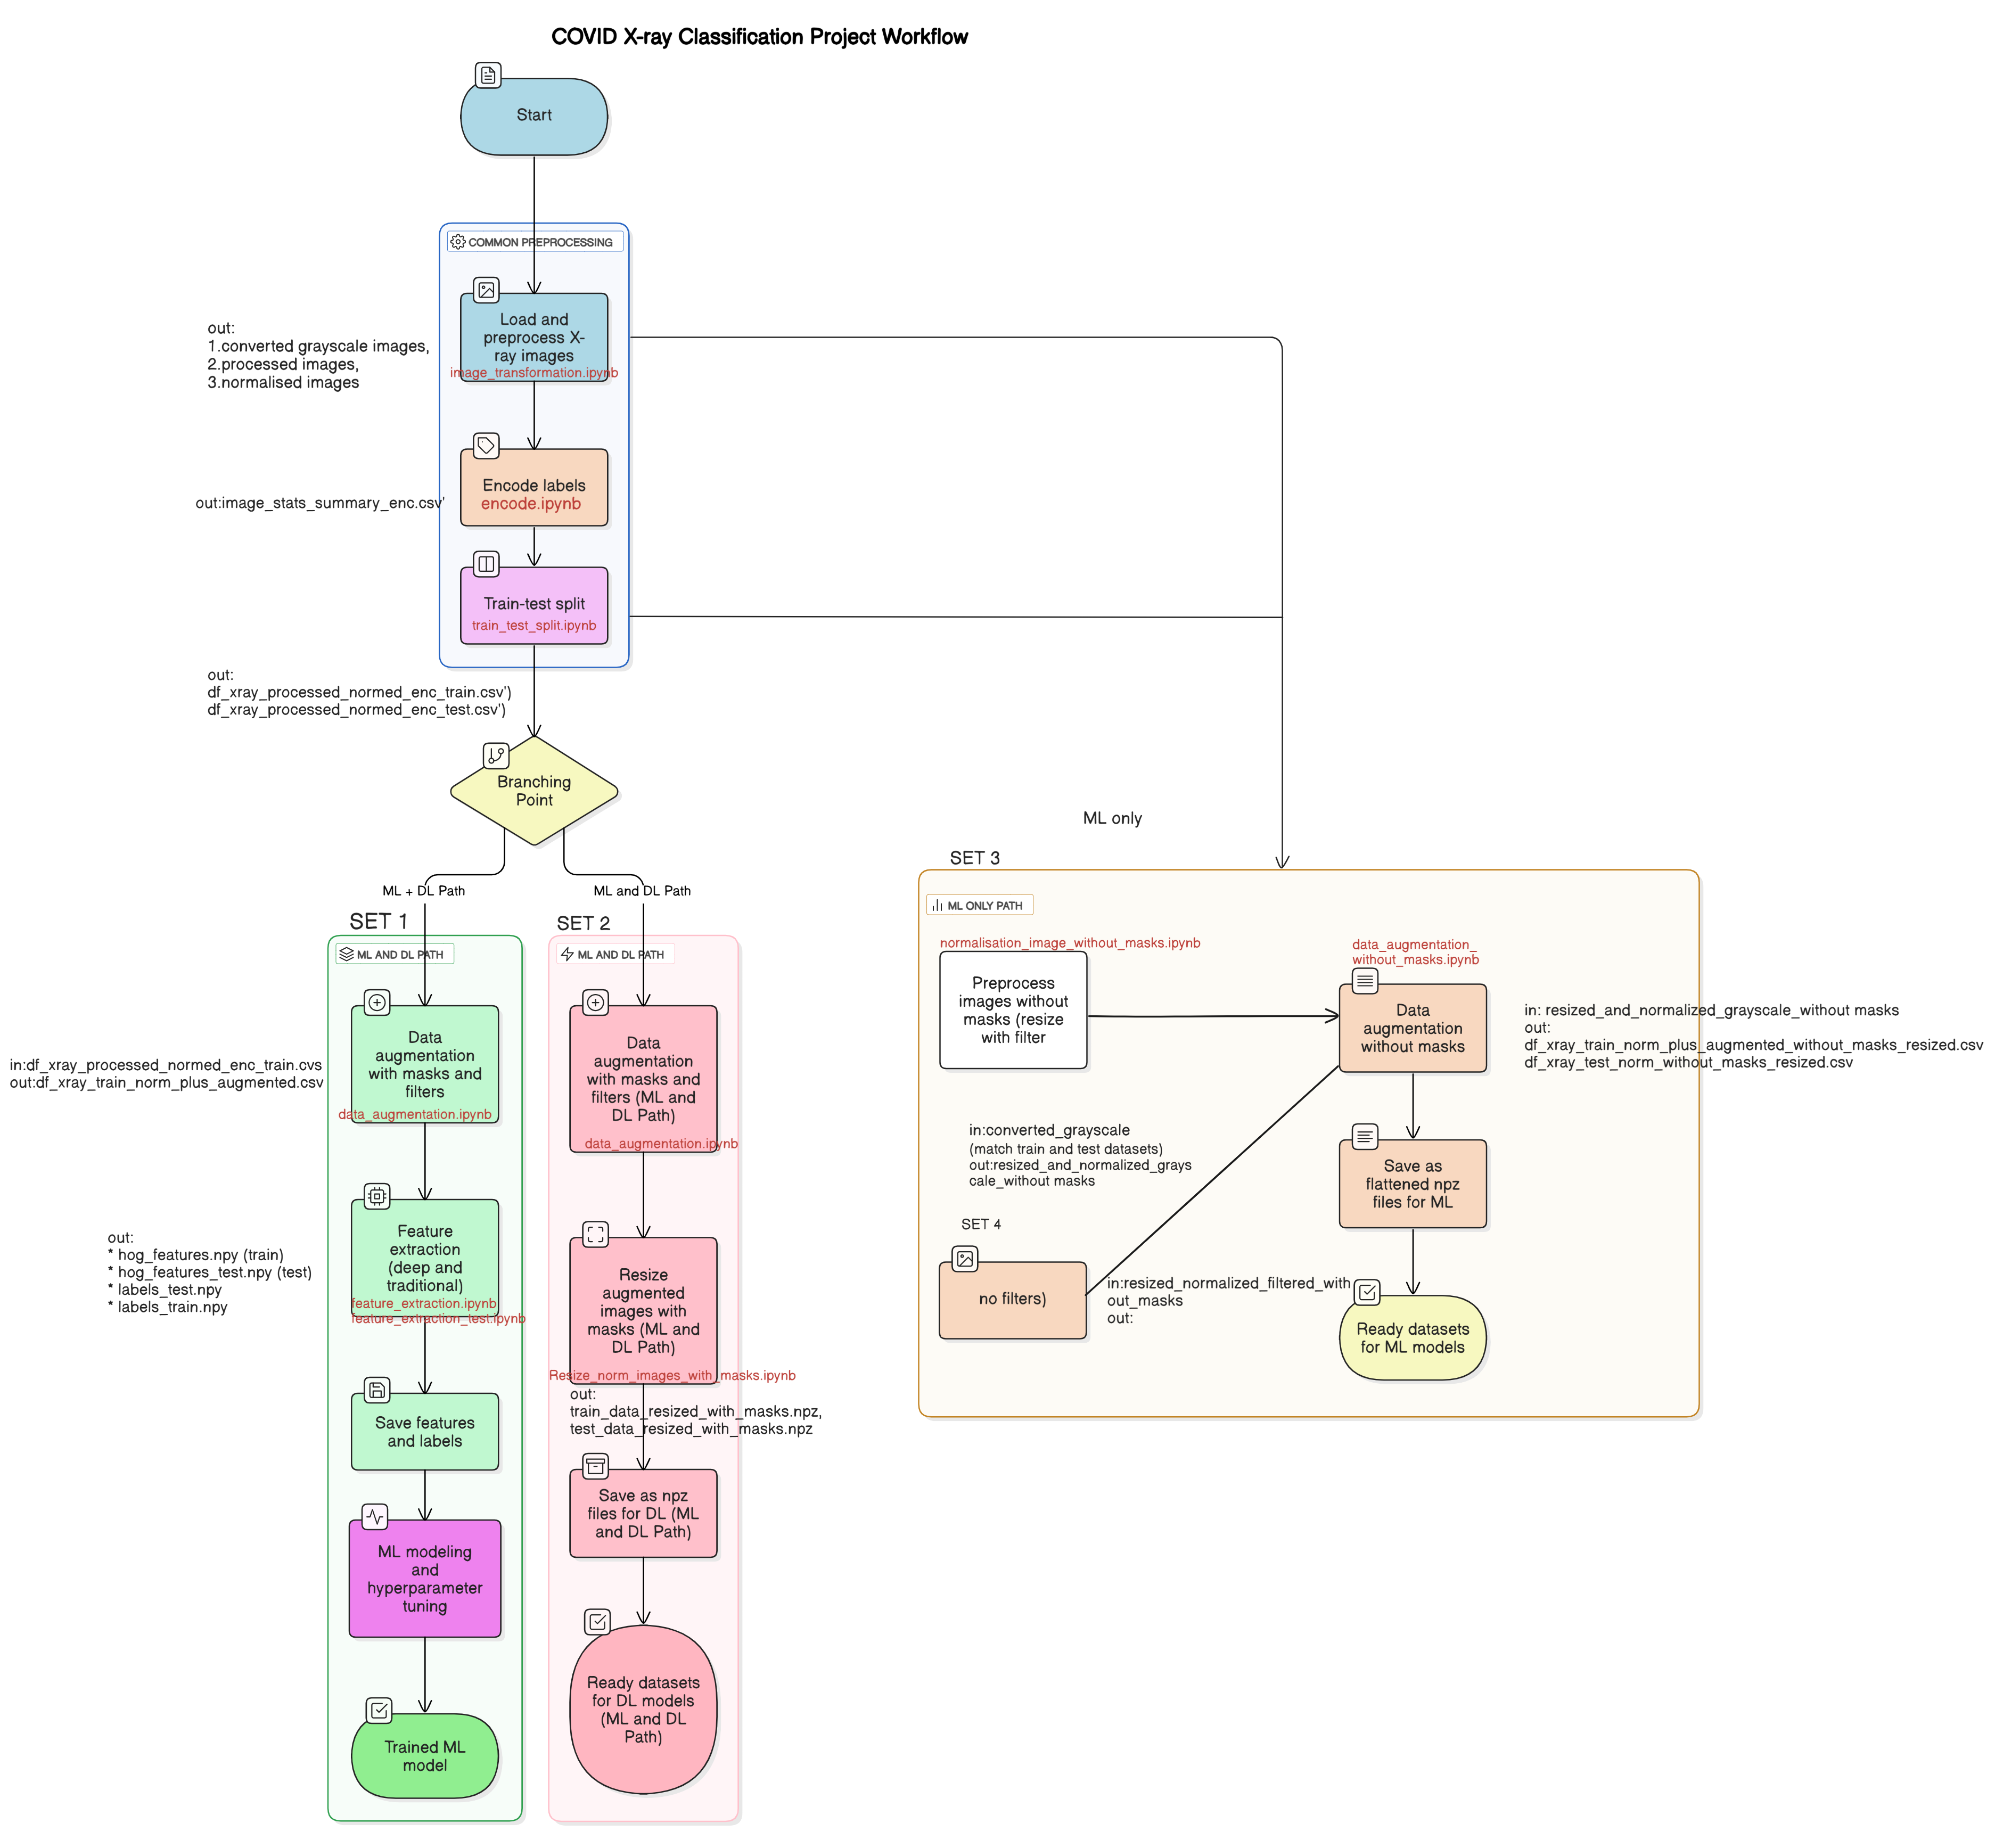
\includegraphics[width=1.0\linewidth]{diagram-export-5-8-2025-4_05_06-PM.png}
    \caption{Sets of images used for ML models}
    \label{fig:WORKFLOW}
\end{figure}
The \textbf{COVID X-ray Classification Project Workflow} outlines the complete pipeline for preparing and modeling chest X-ray data to classify COVID-19 and other conditions using machine learning (ML) techniques.

The process begins with loading and preprocessing the raw X-ray images, where they are converted to grayscale, resized, and normalized using the \texttt{gray\_image.ipynb} script.

Next, labels are encoded into a machine-readable format using \texttt{encode\_labels.ipynb}, and the dataset is split into training and testing sets with \texttt{train\_test\_split.ipynb}.

At this stage, the workflow branches into three sets.

\textbf{SET 1} involves using feature extraction methods such as Histogram of Oriented Gradients (HOG) . The extracted features and labels are saved for model training and hyperparameter tuning.

\textbf{SET 2} applies masks and filters during data augmentation. These images are resized to 128*128 and 20*20 pixels. The augmented images and labels are saved as \texttt{.npz} files for use in ML pipelines.

\textbf{SET 3 } preprocesses images without applying filters by resizing and normalizing them, followed by augmentation without masks. The resulting data is then flattened and stored as \texttt{.npz} files for traditional ML models.

\textbf{SET 4 }preprocesses images after applying filters by resizing and normalizing them.

With this workflow we wanted to ensure a structured and modular approach to data handling, augmentation, feature extraction, and model training.
\\

\subsubsection{Logistic Regression}
We started with logistic regression as it serves as a baseline for performance.Also it is computationally inexpensive and we can quickly iterate over different versions, features, and preprocessing methods.In logistic regression, C is the regularization strength while the solver defines the optimization algorithm.	Regularization helps prevent overfitting (when our model memorizes training data instead of learning patterns).
C is inversely related to regularization:
\begin{itemize}
    \item A smaller C means stronger regularization (simpler model).
    \item A larger C means weaker regularization (more flexible model).
\end{itemize}
Also we need to test different solvers to see which performs best:
\begin{itemize}
    \item liblinear for binary, small-to-medium-sized data.
    \item lbfgs or saga for larger datasets or multi-class problems.
\end{itemize}

\textbf{1st trial}: Hog features(Figure \ref{fig:Logistic_Regression}A).We gave the model HOG features, a fingerprint of edges. This helped the computer guess pretty well.
This model gave an Accuracy of 73.71\%
Overall, best performance, especially for COVID \& Pneumonia.
\\
\textbf{2nd trial}: Images with masks resized(Figure \ref{fig:Logistic_Regression}B)We shrunk the image small and used masks. It didn’t help much.
We got an Accuracy: 58.04\%. The model made bad guesses, especially for Normal and COVID images however Pneumonia class had high recall (0.90) but low precision (0.42).
\\
\textbf{3rd trial}: Images without masks resized without filters(Figure \ref{fig:Logistic_Regression}C)we also fed the model same small images, but now the whole image is visible. This increased the accuracy to 69.24\%  and displayed a nice balance across all disease types.
\\
\begin{figure}[ht] % the [h!] helps force it "here"
    \centering
    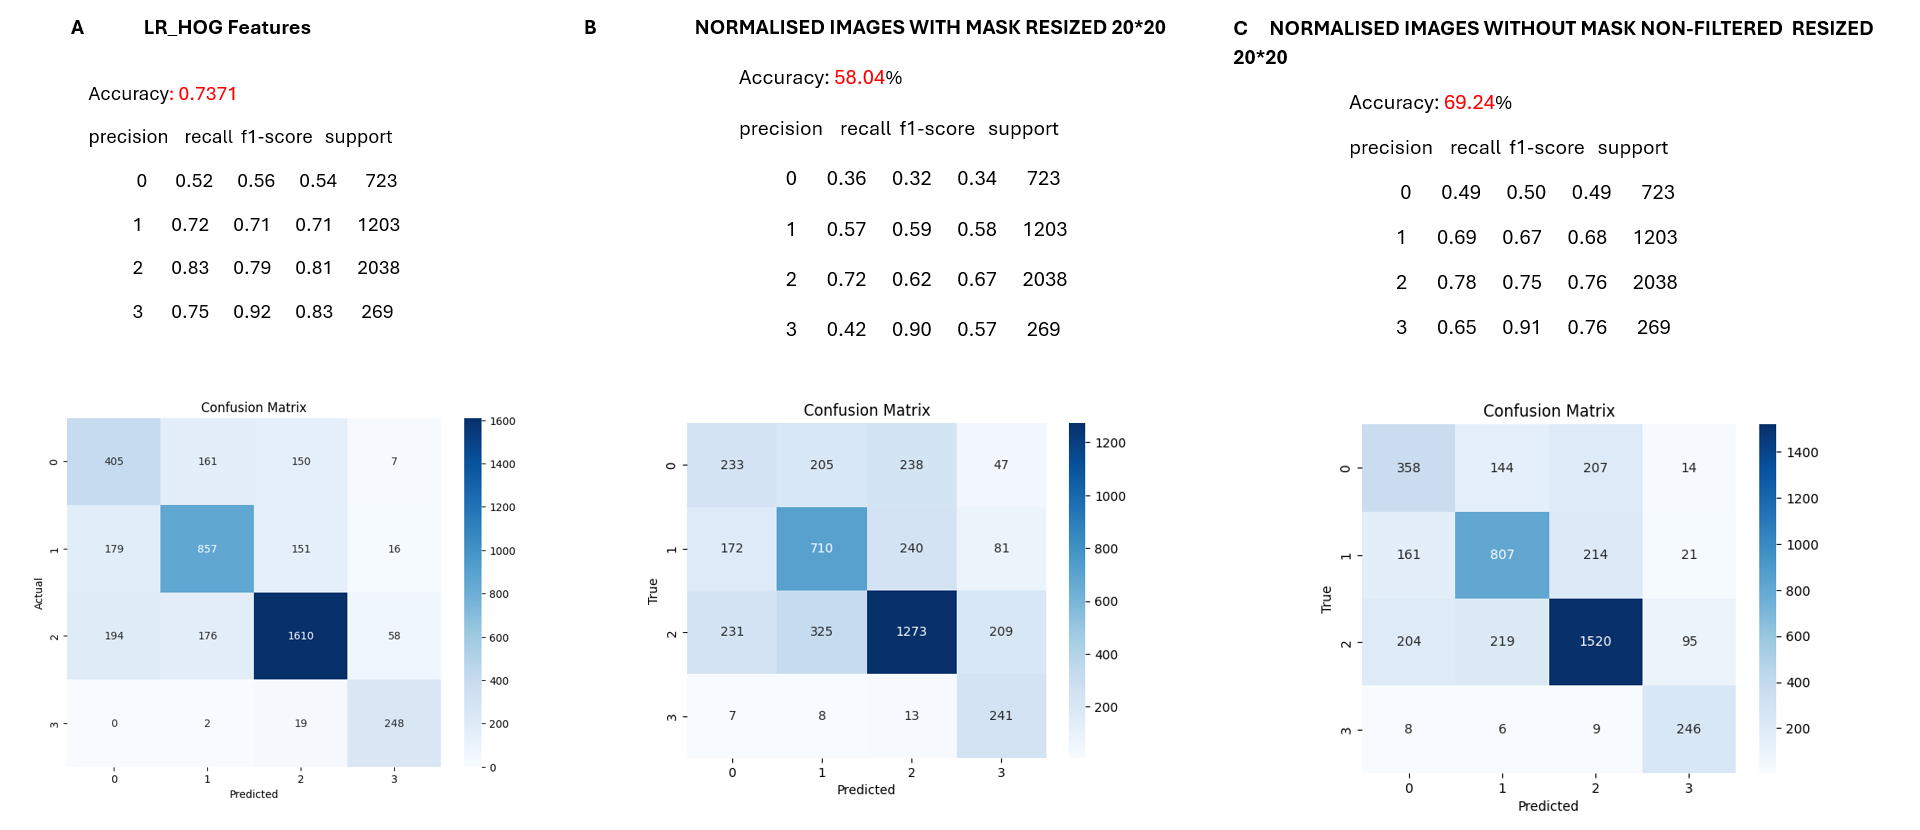
\includegraphics[width=1.0\linewidth]{lr1,2,3.png}
    \caption{Logistic Regression models A, B,C}
    \label{fig:Logistic_Regression}
\end{figure}
\textbf{4th trial}:Random grid search + PCA (Figure \ref{fig:Logistic_Regression_logreg2} A)
While running a GridSearch on HOG features, my system ran out of memory and crashed. To make the training more manageable, I switched to RandomizedSearchCV combined with PCA to reduce dimensionality.
Here we used SAG(Stochastic Average Gradient)which is ideal for large datasets and when we want faster convergence of SGD without noisy updates. It works by iterating through the data in mini-batches. In each iteration,it computes the gradient (slope of the cost function) for each mini-batch, and averages them to update the parameters.Over time, this leads to more stable and faster convergence compared to regular SGD(Stochastic Gradient Descent).Also, for dimensionality reduction PCA was used which reduced features to 100 components.
Using a random grid with PCA we improved the accuracy to 65.37\%, which is solid for logistic regression with HOG characteristics. The best parameters found were C = 0.075, penalty = L1. The PCA retained variance 62\% and showed a better precision-recall balance in COVID class.\\
Class-wise performance: 
\begin{itemize}
    \item Class 2 (2038 samples): Highest F1 (0.74), meaning our model is best at detecting this.
    \item Class 3 (269 samples): Very high recall (0.93) but low precision — it’s over-predicting this class.
    \item Class 0 and 1: More balanced, but weaker F1.
The accuracy drop may be because of the pca which we set to 100.
\end{itemize}

\textbf{5th trials}: Gridsearch cv (Figure \ref{fig:Logistic_Regression_logreg2}B)
We applied Grid Search on normalized, unmasked, non-filtered 20×20 images to obtain the best Params: C=0.1, penalty=L2 and an accuracy of 69.10\%.
Logistic regression after hyperparameter tuning showed slight improvement in accuracy and confusion matrix and displayed a	similar class-wise performance to the base version.The raw HOG features might have contained valuable info that PCA compressed away in the previous model.
\\
\textbf{6th trial}:Manual Parameter Tuning using CuML on HOG features (Figure \ref{fig:Logistic_Regression_logreg2}C).
We then revisited GridSearch with cuML on hog features, which is faster because it uses the GPU.
Here we set solver='qn' in cuML's Logistic Regression (i.e., GPU-accelerated version),and it refers to the Quasi-Newton method.
Quasi-Newton is a family of optimization algorithms used to minimize a function (like the logistic loss).
It is similar in spirit to lbfgs in scikit-learn (also a Quasi-Newton method).It does not support L1 regularization — only L2.
In this experiment, we trained a CuML Logistic Regression model using a subset of the training data (5000 samples) with GPU acceleration to enhance performance. The model utilized \texttt{class\_weight='balanced'} to address class imbalances. This model was fast and efficient and gave the same result as best one (HOG) with an accuracy: 73.47\% on the test set.

The classification report reveals that the model's recall is highest for the Normal (2) class (85\%)and Viral Pneumonia (3) (82\%), while the lowest recall is for COVID (0) (39\%). The precision and F1-scores also reflect this imbalance, with the model performing better on the more frequent classes.
\\
Summary:
\begin{itemize}
    \item HOG features yielded the best accuracy (~73.7\%) with strong recall on Pneumonia and COVID.
    \item Raw pixel features (even when resized) underperformed compared to HOG or PCA-based features.
    \item PCA compressed HOG features to retain 62\% variance, resulting in slightly reduced performance but possibly lower model complexity.
    \item Logistic regression benefited modestly from hyperparameter tuning (Grid and Random Search), but improvements were incremental.
    \item Pneumonia class consistently showed high recall but variable precision.
\end{itemize}
In conclusion , the Logistic Regression Model on hog features with Best C: 0.01 obtained by performing manual tuning using Cuml gave us the best accuracy (73\%)
Room for Improvement: Logistic regression might not be the best choice for such a high-dimensional feature set. Therefore we next chose to experiment with other models like Support Vector Machines (SVM) and Random Forests, which could perform better without requiring dimensionality reduction.


\begin{figure}[h!] % the [h!] helps force it "here"
    \centering
    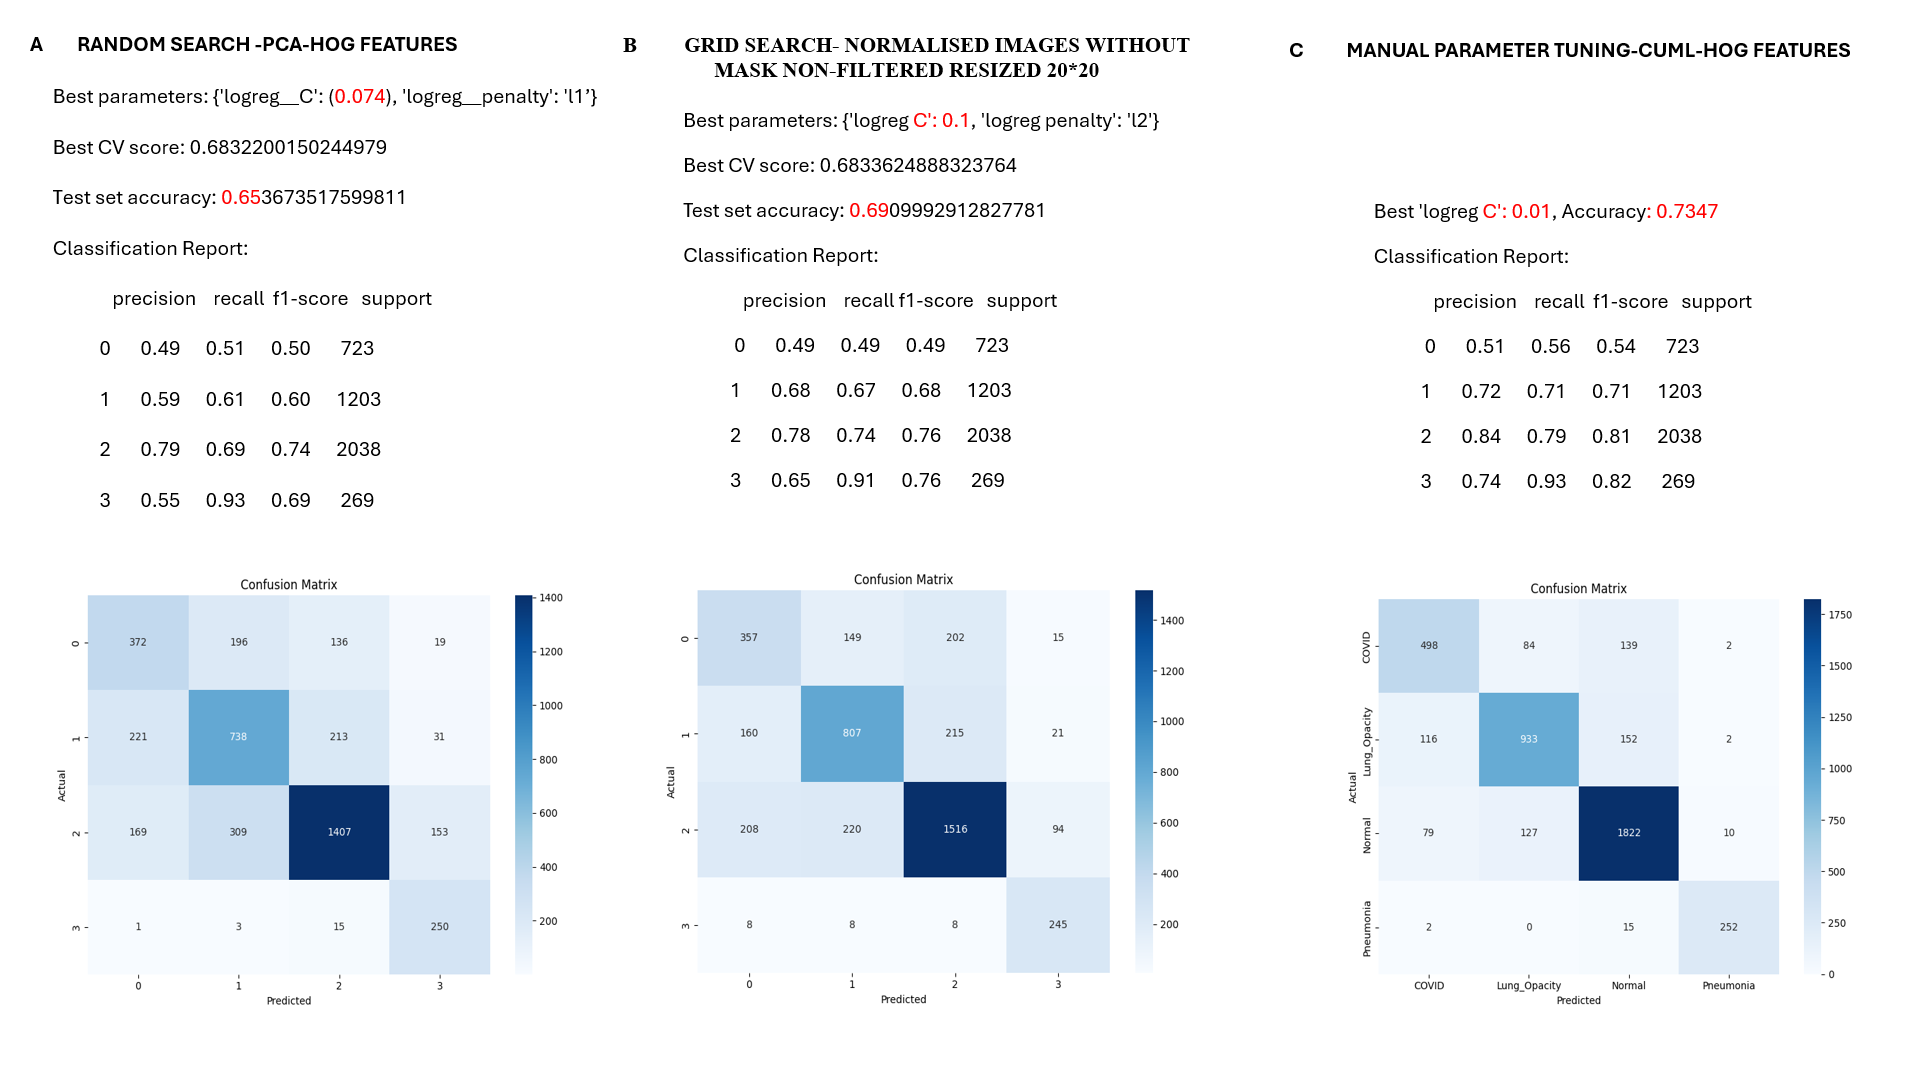
\includegraphics[width=1.0\linewidth]{logreg2,a,b,c.png}
    \caption{More Logistic Regression models A, B,C}
    \label{fig:Logistic_Regression_logreg2}
\end{figure}


\subsubsection{Random Forst}
\colorbox{yellow}{ToDO Alex}

\subsubsection{SVM}
Linear SVM
\begin{itemize}
    \item Separates data using a straight line (in 2D) or a hyperplane (in higher dimensions).
    \item Assumes that the data is linearly separable (i.e., classes can be separated by a straight boundary).
    \item Uses a linear kernel.
    \item Fast and efficient for high-dimensional, sparse data like text or HOG features.
\end{itemize}
Good for: When the data has clear linear boundaries.\\
\\
Nonlinear SVM 
\begin{itemize}
    \item Can separate data with curved or complex boundaries.
    \item Uses kernel tricks (e.g., RBF, polynomial) to map the data into higher dimensions where it may become linearly separable.
    \item More flexible but computationally expensive, especially on large datasets.
Good for: Data where classes are intertwined and not separable by a straight line.
\end{itemize}
\textbf{1th trial } \colorbox{yellow}{ToDo Yvonne}\\ 
\textbf{2th trial } \colorbox{yellow}{ToDo Yvonne}\\
\textbf{3th trial } \colorbox{yellow}{ToDo Yvonne}\\
\textbf{4th trial }SGDClassifier(Linear SVM) + HOG (With hyperparameter search) Figure \ref{fig:SVM_MODELS}A. SGD still supports hinge loss, so it behaves like a linear SVM and also Supports L1, L2, ElasticNet regularization.In this model we used Randomized searchCV best estimator pipeline(Standandr Scaler,PCA, SGD classifier). \begin{verbatim}
Best Hyperparameters found were:
{'clf__penalty': 'l1', 'clf__learning_rate': 'optimal', 'clf__alpha': 0.001}
\end{verbatim}
We observed low overall accuracy (56.89\%),however the recall for the COVID class (class 0) was better at 63.07\%, and even stronger for Viral Pneumonia (class 3) at 86.62\%.\\
Perhaps Linear models like SGDClassifier may not fully capture complex patterns.
Therefore, the next steps would be to :
\begin{itemize}
    \item try a Tree-based Model eg. XGBoost or LightGBM which handle non-linear relationships well and work directly on HOG features (no need to resize images)
    \item experiment with non-linear SVM on a subset of our data (e.g., 2–5k images) to test potential gains
\end{itemize}
\textbf{5th trial }So the next model we tested was grid search on nonlinear SVM using kernel rbf using a smaller dataset (5000) of hog features.(Figure \ref{fig:SVM_MODELS}B)We performed grid search with reduced parameter space.The Accuracy improved to 72\%, and we found the Best parameters: \texttt{svc\_ C= 1},\texttt {svc\_ gamma = scale}.
\\
\begin{figure}[h!] % the [h!] helps force it "here"
    \centering
    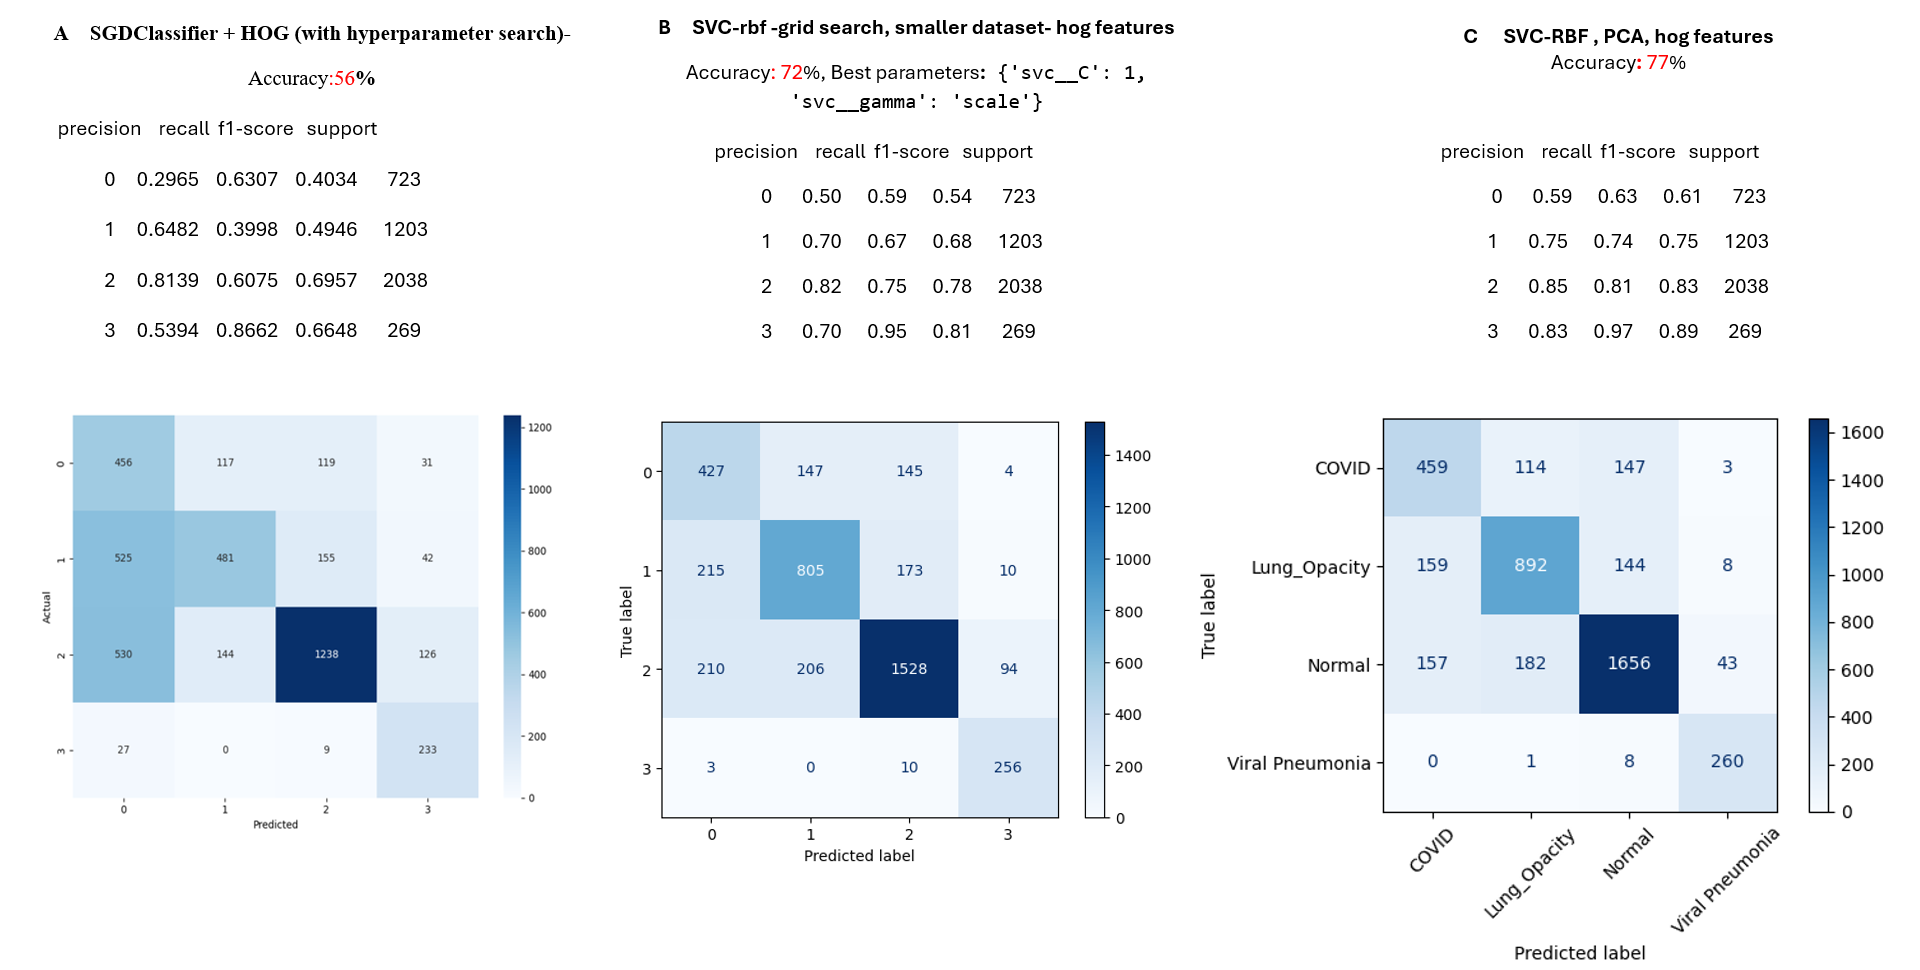
\includegraphics[width=1.0\linewidth]{svm ABC.png}
    \caption{SVM MODELS}
    \label{fig:SVM_MODELS}
\end{figure}
\textbf{6th trial }Since SVC\- RBF kernel gave us better results we decided to run it on hog features after dimensionality reduction using PCA.TWe observed an accuracy of 77\%.The Cumulative explained variance for PCA by 200 components was 62.06\%. However the precision and recall for class 0 did not show much improvement and therefore, we proceeded with other ML models.\\


In conclusion, the SVC model with RBF kernel on Hog features with PCA dimensionality reduction gave us the best accuracy of 77\%.

\subsubsection{XGBoost}
\colorbox{yellow}{ToDo Yvonne}

\subsubsection {DENSE NETWORKS: MLP-Classifier} 
\colorbox{yellow}{Does this belong to the machine learning? Or is it Deep learning?}\\
\colorbox{yellow}{But from what we have done with the input data, it suits more to the machine learning part. don't know.}\\
\colorbox{yellow}{It is somehow inbetween?!!}\\
 Multi-Layer Perceptron, which is a classic feedforward neural network consists of: An input layer, One or more hidden layers (each with fully connected / dense neurons) and an output layer.Each neuron in a layer is connected to every neuron in the next layer which makes it a dense network.\\
 
\textbf{1st trial }\\We trained an MLPClassifier (Multi-layer Perceptron) using HOG features.the first MLP classsifer had the following architecture:sequential 3 dense layers: 512, 256, 128 neurons, ReLU activation + dropout, model compiled using adam optimizer and categorical crossentropy loss.This gave us solid result for a first MLP on HOG features — 78\% accuracy with especially strong recall on Viral Pneumonia (97\%).
In the next trial we improved this further by making improvements to the model architecture.\\

\textbf{2nd trial }\\
We increased the number of layers/neurons to make deeper network(Sequential layers: 1024, 512 , 256
and performed BatchNormalization before activations for more stable training, implemented EarlyStopping + ReduceLROnPlateau for smarter training.
The overall accuracy of this model was 76.99 \%, which is a notable boost from previous models.However, COVID (0) is still the weakest class (59\% precision and recall), indicating the model struggles with it — possibly due to class imbalance or feature overlap.Lung Opacity (1) shows consistent, decent performance (75\% recall). Normal (2) displayed the strongest precision (85\%) and recall (82\%), showing good separability.Viral Pneumonia (3) displayed excellent recall (96\%) as it had very few false negatives.\\

\textbf{3rd trial }\\
The next trial  we tried an updated MLP classifier with an edition of Class weights to Boost minority class (COVID) explicitly, and activation function Leaky Relu to avoid dead neurons, in addition to previous additions. The key changes made were:
 \begin{itemize}
     \item LeakyReLU with alpha=0.1 helps mitigate dead neurons by allowing a small gradient when the input is negative.
     \item Dropout with rates of 50\% after the first layer and 30\% after the second layer helps prevent overfitting by randomly dropping out neurons during training.
     \item Adam optimizer with a smaller learning rate (0.0005) to help avoid overshooting the minima during training.
     \item Class weights are computed to handle class imbalance (especially important for class 0 - COVID).
     \item Batch Normalization is included after each layer to stabilize the learning process
\end{itemize}
The accuracy is now 0.7817, which is a noticeable improvement from the previous attempts.Looking at the confusion matrix, we can observe: Class 0 (COVID) has lower precision and recall than the other classes. This could mean our model is having difficulty distinguishing between COVID and other classes (maybe due to class imbalance).Classes 1 (Lung Opacity), 2 (Normal), and 3 (Viral Pneumonia) are being classified well, with high F1-scores and balanced precision and recall.\\

\textbf{4th trial }\\
In this model we appliesd SMOTE to help balance the class distribution by generating synthetic samples for the minority classes (Class 0 - COVID), which can help the model learn better representations for those classes.We later scaled the resampled features using 50 epochs, Smaller batch size (32), early stopping, to prevent overfitting, and trained the model on the new balanced data (without class weights). Although the model gave consistent ~77.7–78\% accuracy, we observed good precision and recall for class 2 and 3 however class 0 is still underperforming.\\

\textbf{5th trial }\\
In this model we tried focal loss which is particularly useful when we're dealing with class imbalance, as it puts more focus on hard-to-classify examples.We used a gamma of 2.0 and alpha of 0.25 — good defaults based on the original focal loss paper. Class 0 is still underperforming slightly (precision = 0.60, recall = 0.58), meaning it's being confused with other classes. This is likely due to it having fewer or noisier samples or its features overlapping with class 1.Class 2 and 3 are performing very well, especially class 3 (recall = 0.93) — so the model is confidently identifying these.\\

\textbf{6th trial }\\
We next tried MLP on ResNet features.ResNet (Residual Networks) is a deep convolutional neural network pretrained on ImageNet.It learns hierarchical, high-level features (like textures, shapes, patterns) that are often more effective than handcrafted ones.Extracting features from a pretrained ResNet and feeding them into a simple MLP can boost performance, especially for medical images.
The model performed very well with an overall Accuracy of 82.8\%, COVID Recall: 69\%, Lung Opacity Recall: 78\%,    Normal Recall: 89\%,Pneumonia Recall: 94\%.This matrix shows that:Normal and Pneumonia classes are classified with high confidence.COVID and Lung Opacity occasionally get confused with each other and with Normal.
Our current results are strong enough that it makes perfect sense to move to deep learning or CNN-based models next.
\begin{figure}[ht] % the [h!] helps force it "here"
    \centering
    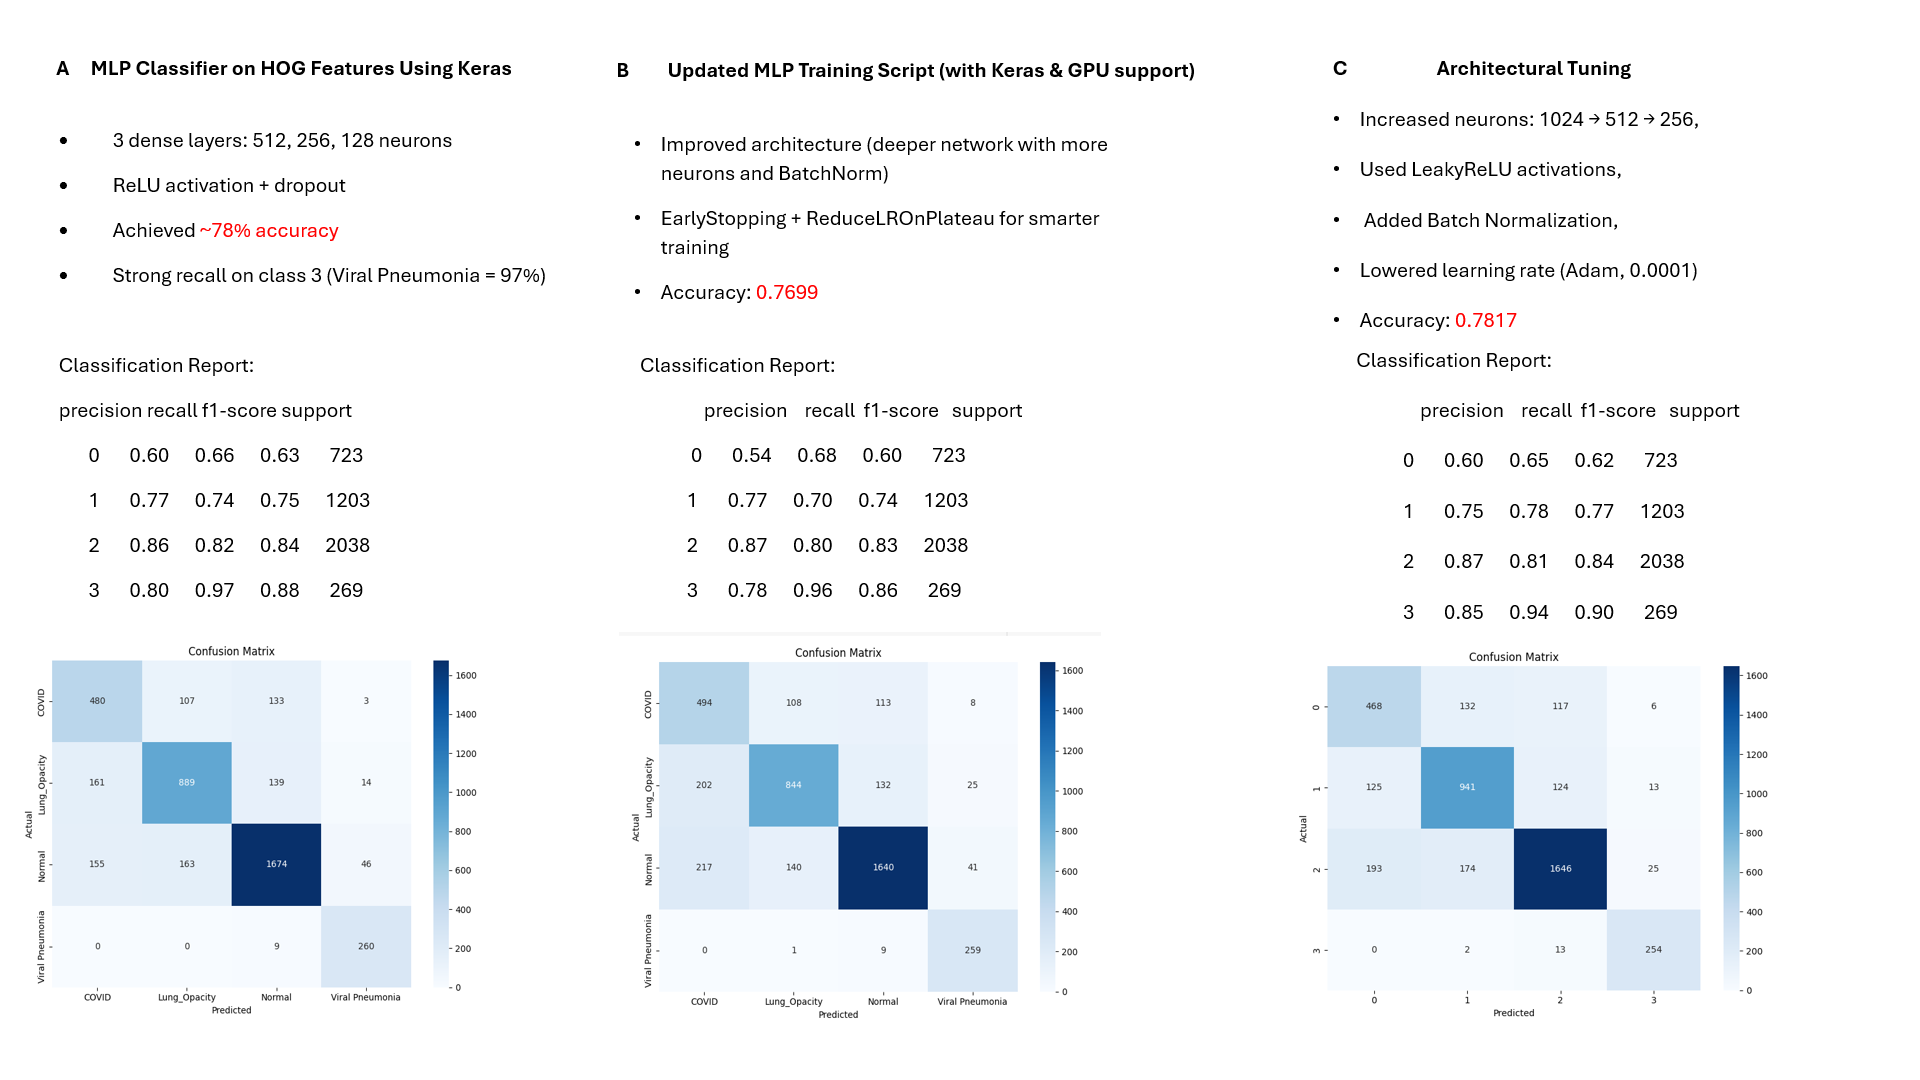
\includegraphics[width=1.0\linewidth]{mlpclassifier a,b,c.png}
    \caption{MLP CLASSIFIER A, B, C}
    \label{fig:MLP_CLASSIFIER}
\end{figure}
We wanted to see how the MLP classifier model was learning our data anad so we decided to plot the accuracy and loss per epochs for the first trial and the last(figure \ref{fig:MLP_CLASSIFIER_compare}). On analysis of figure \ref{fig:MLP_CLASSIFIER_compare}a (20 epochs) we found training Loss decreases steadily suggesting the model is learning from the training data.
The Validation Loss Plateaus and then increases after epoch ~6–7 which suggests overfitting.The model training Accuracy rises to ~0.95 which is excellent however the validation Accuracy flatlines around 0.83–0.84 which showed that the model is not improving on unseen data.
Figure \ref{fig:MLP_CLASSIFIER_compare}b (8 epochs) showed a similar trend, just shorter duration. We obeserved still a gap between training and validation performance (train ~0.93 vs val ~0.83).The validation loss increases even earlier suggesting overfitting happens faster.\\
These resulsts show that Resnet features wrok well and MLP learns effectively on the training data.However we observe overfitting whih needs to be fixed.\\
\textbf{7th trial }\\
To address this we next try to add L2 regularization to Dense layers that helps reduce overfitting by penalizing large weights, increase dropout slightly (0.4) that increases regularization by randomly dropping neurons during training and use early stopping that avoids overfitting by halting training when the model stops improving on validation data.We also try reducing the number of neurons (e.g., 256 → 128 → 64) to avoid overfitting and consider adding BatchNormalization after dense layers.
\begin{figure}[ht] % the [h!] helps force it "here"
    \centering
    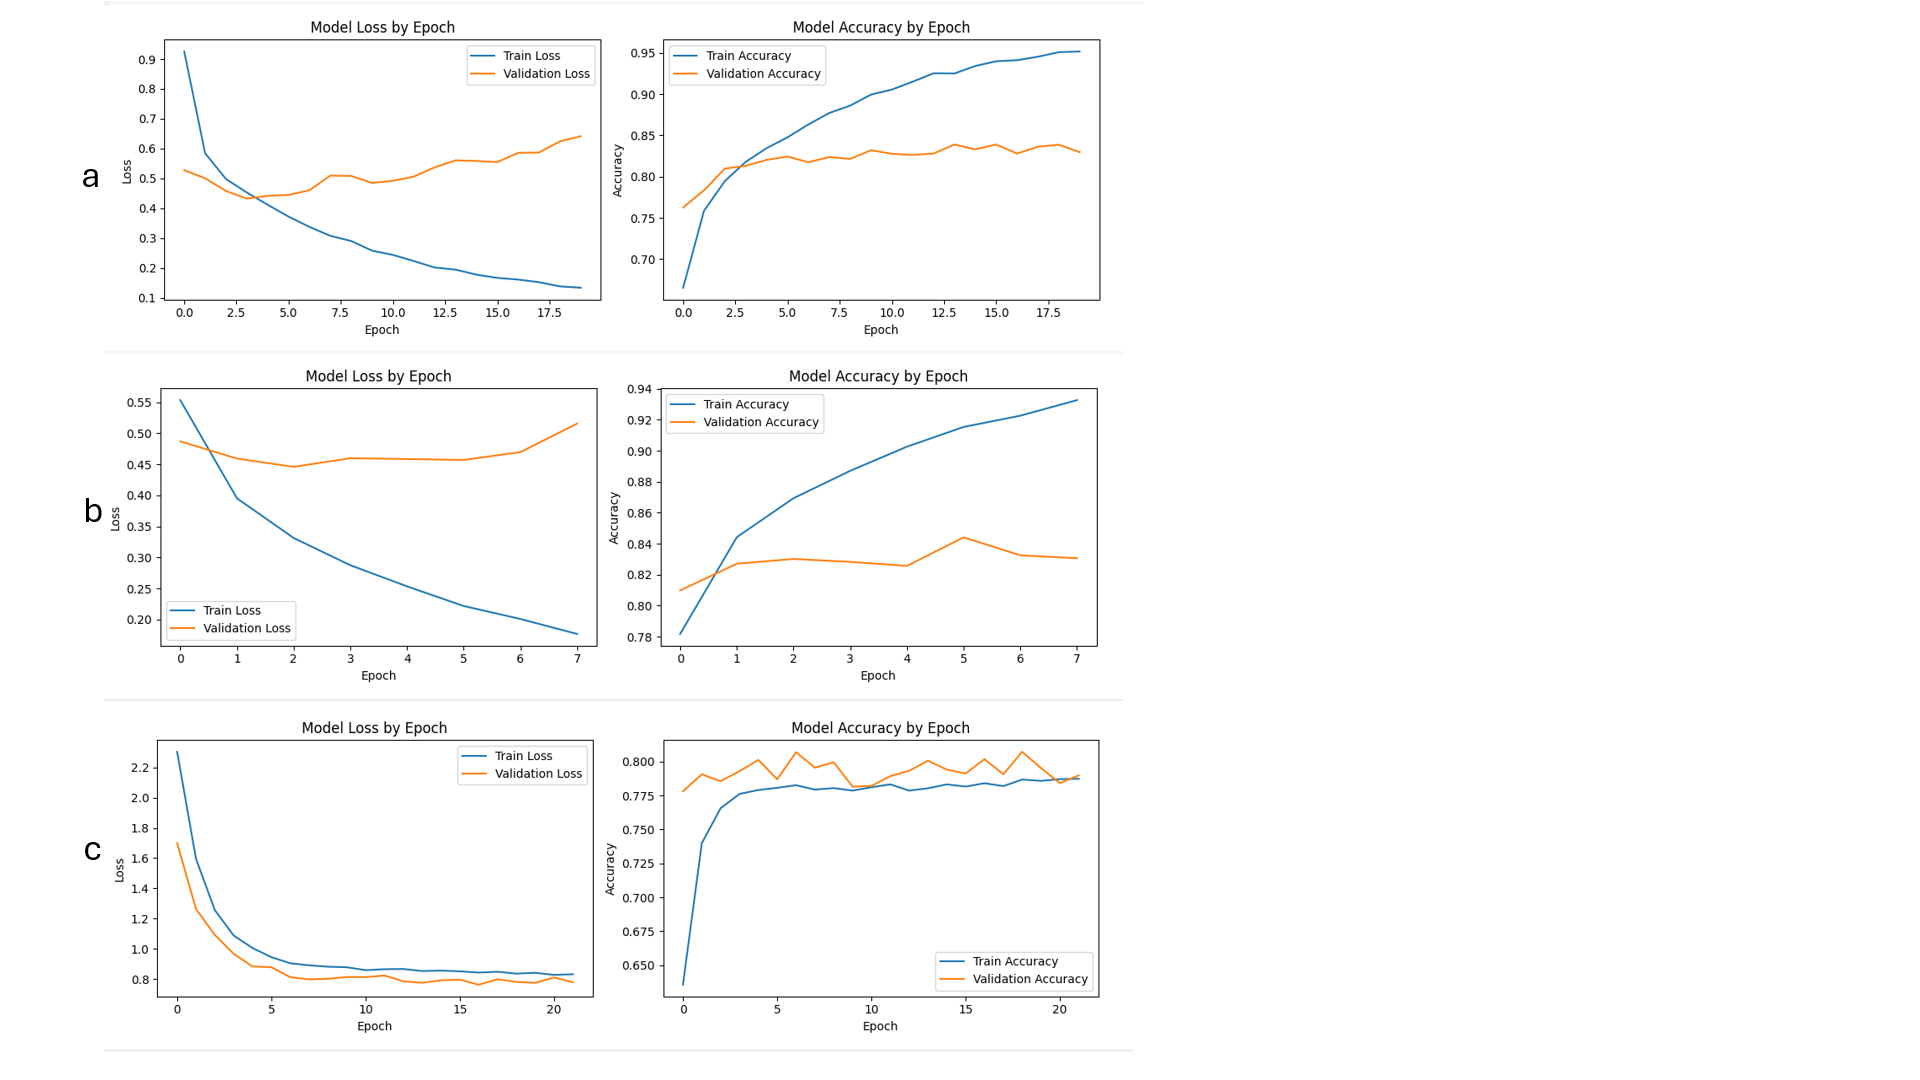
\includegraphics[width=1.0\linewidth]{comparemlp2.png}
    \caption{MLP CLASSIFIER A, B, C}
    \label{fig:MLP_CLASSIFIER_compare}
\end{figure}
Loss and Accuracy Plot Interpretation of figure \ref{fig:MLP_CLASSIFIER_compare}c shows that both training and validation loss drop significantly in the first few epochs and stabilize around epoch 10.The gap between training and validation loss is small, which means low overfitting.Accuracy rises quickly and stabilizes around 78–80\% for both training and validation, showing consistent learning and generalization.
The validation accuracy occasionally surpasses training accuracy, likely due to dropout and regularization.

The Classification Report showed an overall accuracy of 75\% over 4,233 samples which is solid for a multi-class task.
Class 2 (largest class): Strong performance (F1 = 0.83), suggesting the model is very confident in this class.
Class 1: Also good (F1 = 0.72).
Class 0: Weaker (F1 = 0.56), possibly due to overlapping features.
Class 3: Interesting — high recall (0.98) but lower precision, suggesting the model predicts this class a lot, possibly overgeneralizing to it.\\
\\
In conclusion, MLP Classifier on ResNet Features gave us the best accuracy(82\%).Since class 0 still remians a probelm moving to a Convolutional Neural Network (CNN) is the logical next step, since were working with image data (X-rays), and traditional ML models like SVMs or MLPs (even with augmentation and tuning) may struggle to capture spatial hierarchies and localized patterns critical for medical imaging.\\

\section{Deep Learning}

\subsection{Prepare Data for Deep Learning}
\colorbox{yellow}{To Do: As we might have a different preprocessing pipeline we have to }\\
\colorbox{yellow}{describe preprocessing of data we did for deep learning.}\\

\subsection{Metrics to Evaluate the Model Results}
Do we need this subsection again for DL or is it the same as for ML. 
Maybe we can delete this subsection later.

Grad-CAM?

\subsection{Modelling and Results}
\subsubsection{Model 1 --> To be replaced with a name}
This could be a CNN without transfer learning which Alex is working with. 

\subsubsection{Model 2 --> To be replaced with a name}
This could be a pretrained model.

\subsubsection{Model 3 --> To be replaced with a name}
This could be a pretrained model.


\section{Conclusion}

Overall Conclusion
Which model performed best
What worked, what did not work? Why?

\section{Example include image and table - To be removed at the end}

Put images you want to include to this report in the subfolder: figures\_report\_2 and use relative paths inside this report.
Upload them on git aswell.

\begin{figure}[ht] % the [h!] helps force it "here"
    \centering
    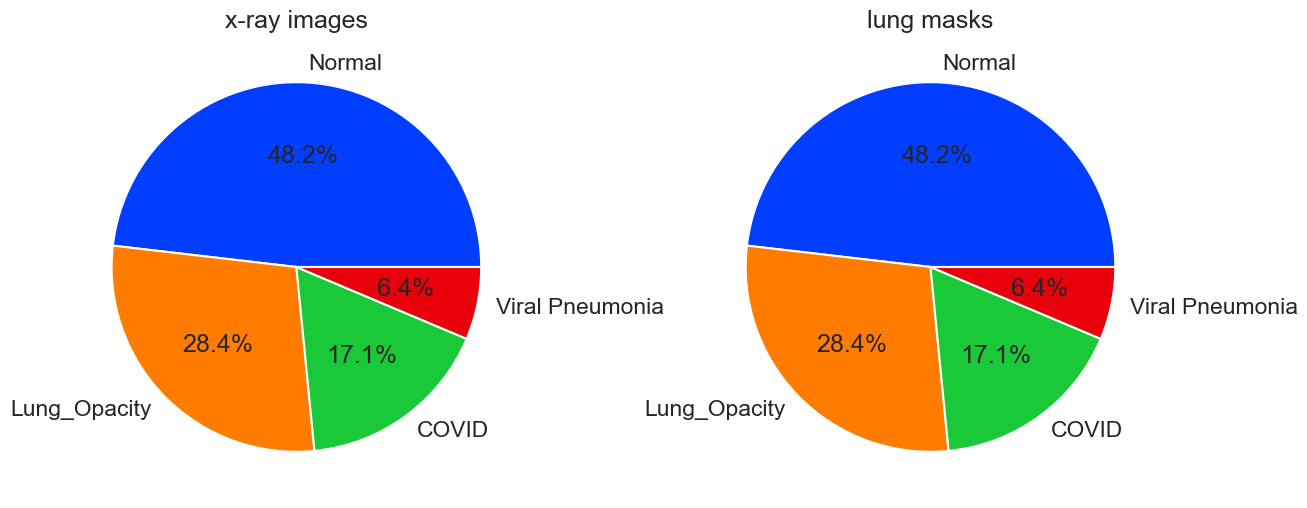
\includegraphics[width=1.0\linewidth]{../figures/figures_report_2/classes.png}
    \caption{Examples of image}
    \label{fig:example_image}
\end{figure}

Figure \ref{fig:example_image} shows ...


\begin{table}[ht]
    \centering
    \begin{tabular}{|c|c|c|}
        \hline
        \textbf{X} & \textbf{Y} & \textbf{Z} \\ \hline
        1 & 2 & 3 \\ \hline
        4 & 5 &  \\ \hline \hline
        6 &  & 7 \\ \hline
    \end{tabular}
    \caption{Example of table}
    \label{tab:example_table}
\end{table}

Table \ref{tab:example_table} shows \dots

\end{document}